%%%%%%%%%%%%%%%%%%%%%%%%%%%%%%%%%%%%%%%%%%%%%%%%%%%%%%%%%%%%%%%%%%%%%%%%

%%% LaTeX Template for ECAI Papers
%%% Prepared by Ulle Endriss (version 1.0 of 2023-12-10)

%%% To be used with the ECAI class file ecai.cls.
%%% You also will need a bibliography file (such as mybibfile.bib).

%%%%%%%%%%%%%%%%%%%%%%%%%%%%%%%%%%%%%%%%%%%%%%%%%%%%%%%%%%%%%%%%%%%%%%%%

%%% Start your document with the \documentclass{} command.
%%% Use the first variant for the camera-ready paper.
%%% Use the second variant for submission (for double-blind reviewing).

\documentclass{ecai}
%\documentclass[doubleblind]{ecai}

%%%%%%%%%%%%%%%%%%%%%%%%%%%%%%%%%%%%%%%%%%%%%%%%%%%%%%%%%%%%%%%%%%%%%%%%

%%% Load any packages you require here.

\usepackage{latexsym}
\usepackage{amssymb}
\usepackage{amsmath}
\usepackage{amsthm}
\usepackage{booktabs}
\usepackage{enumitem}
\usepackage{graphicx}
\usepackage{color}
\usepackage{tikz} % Added TikZ package for diagrams
\usepackage{algorithm} % Added for algorithm environment
\usepackage{algpseudocode} % Added for algorithmic environment

%%%%%%%%%%%%%%%%%%%%%%%%%%%%%%%%%%%%%%%%%%%%%%%%%%%%%%%%%%%%%%%%%%%%%%%%

%%% Define any theorem-like environments you require here.

\newtheorem{theorem}{Theorem}
\newtheorem{lemma}[theorem]{Lemma}
\newtheorem{corollary}[theorem]{Corollary}
\newtheorem{proposition}[theorem]{Proposition}
\newtheorem{fact}[theorem]{Fact}
\newtheorem{definition}{Definition}

%%%%%%%%%%%%%%%%%%%%%%%%%%%%%%%%%%%%%%%%%%%%%%%%%%%%%%%%%%%%%%%%%%%%%%%%

%%% Define any new commands you require here.

\newcommand{\BibTeX}{B\kern-.05em{\sc i\kern-.025em b}\kern-.08em\TeX}

%%%%%%%%%%%%%%%%%%%%%%%%%%%%%%%%%%%%%%%%%%%%%%%%%%%%%%%%%%%%%%%%%%%%%%%%

\begin{document}

%%%%%%%%%%%%%%%%%%%%%%%%%%%%%%%%%%%%%%%%%%%%%%%%%%%%%%%%%%%%%%%%%%%%%%%%

\begin{frontmatter}

%%% Use this command to specify your submission number.
%%% In doubleblind mode, it will be printed on the first page.

\paperid{123}

%%% Use this command to specify the title of your paper.

\title{Masala Mamu : Agentic AI Kitchen Assistant}

%%% Use this combinations of commands to specify all authors of your
%%% paper. Use \fnms{} and \snm{} to indicate everyone's first names
%%% and surname. This will help the publisher with indexing the
%%% proceedings. Please use a reasonable approximation in case your
%%% name does not neatly split into "first names" and "surname".
%%% Specifying your ORCID digital identifier is optional.
%%% Use the \thanks{} command to indicate one or more corresponding
%%% authors and their email address(es). If so desired, you can specify
%%% author contributions using the \footnote{} command.
\author[A,B]{\fnms{Barani}~\snm{Ranjan S}}
\author[A,B]{\fnms{Brijgopal}~\snm{Bharadwaj}}
\author[A,B]{\fnms{M Chandan Kumar}~\snm{Rao}}
\author[A,B]{\fnms{Shunmuga}~\snm{Janani A}}
\author[A,B]{\fnms{Siva}~\snm{S}}
\address[A]{Division of Interdisciplinary Sciences}
\address[B]{Indian Institute of Science, Bangalore}
%%% Use this environment to include an abstract of your paper.

\begin{abstract}
In the evolving landscape of smart homes, modern households face increasing complexity in managing day-to-day kitchen operations, including grocery tracking, meal planning, dietary health monitoring, and budget optimization. This project introduces the Agentic AI-Powered Kitchen Assistant, an intelligent, multi-agent system that automates and augments household kitchen management using the latest advancements in artificial intelligence, multimodal natural language processing, and external API integrations. At the core of this system is a Router Agent (built using LangChain/LangGraph) that dynamically delegates tasks to specialized agents based on user queries and contextual requirements. These agents include:
Inventory Manager Agent: Maintains a real-time inventory by interfacing with a database and updates stock levels as items are consumed or added. Price Comparison \& Ordering Agent (MCP): Connects to multiple vendor APIs to identify cost-effective purchasing options and initiate grocery orders. Recipe Generator Agent: Using the current inventory and user preferences, we propose recipes that are nutritious and tailored to dietary restrictions. Health \& Diet Chart Agent: Tracks nutritional intake and provides personalized insights via a dashboard backed by dietary guidelines.
The system communicates with a central LLM (Large Language Model) which facilitates natural language understanding and reasoning, bridging user intent with agent actions. The assistant supports multimodal NLP, allowing users to interact using both speech-to-text and text-based commands.

\end{abstract}

\end{frontmatter}

\section{Introduction}

The increasing complexity of maintaining a balanced diet while being cost-conscious presents a significant challenge for many households. Existing solutions typically address either nutrition tracking or price comparison separately, creating a fragmented user experience. Masala Mamu bridges this gap by offering an integrated approach to meal planning and grocery shopping, with a focus on the Indian context where diverse dietary preferences and a complex e-commerce landscape make optimized food decisions challenging.

The key contributions of this project include:
\begin{itemize}[noitemsep,topsep=0pt]
    \item A multi-agent architecture that intelligently routes user queries to specialized agents
    \item A nutrition analysis system that provides detailed macro-nutrient breakdowns for recipes and ingredients
    \item A price comparison engine that scrapes and compares grocery prices across major Indian e-commerce platforms
    \item An inventory management system with vision-based ingredient recognition and semantic search capabilities
    \item A real-time nutrition tracking dashboard with visualizations and personalized insights
\end{itemize}

\section{System Architecture}

\subsection{Multi-Agent Architecture}

Masala Mamu employs a modular architecture comprised of specialized agents coordinated by a central routing mechanism. As illustrated in Figure 1, the system consists of:

\begin{figure}[h]
\centering
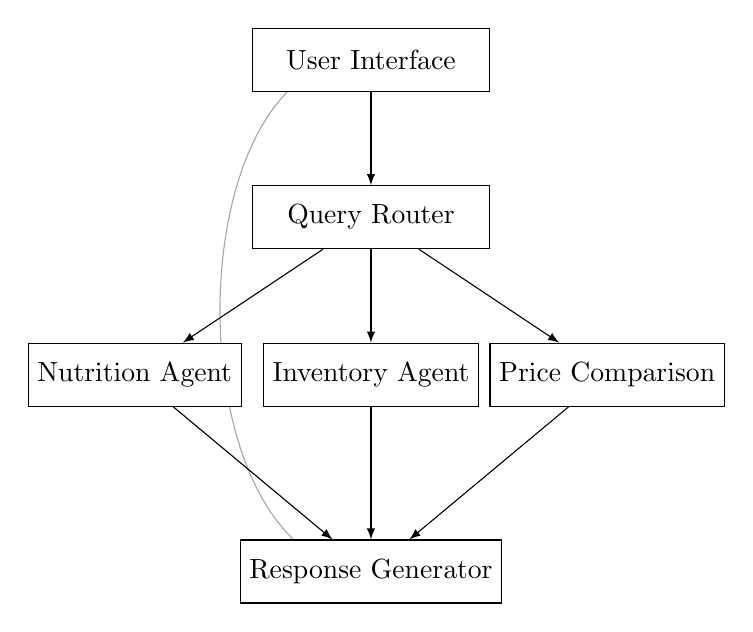
\begin{tikzpicture}[>=latex] % Use latex arrow style which is very clear

    % Draw the curved arrow first (will be behind everything)
    \draw[->, gray!70, thin] (0,-6.5) to[out=180,in=180] (0,0);

    % Define the nodes with opaque backgrounds and borders
    \node[rectangle, draw, fill=white, minimum width=3cm, minimum height=0.8cm] (user) at (0,0) {User Interface};
    \node[rectangle, draw, fill=white, minimum width=3cm, minimum height=0.8cm] (router) at (0,-2) {Query Router};
    \node[rectangle, draw, fill=white, minimum width=2cm, minimum height=0.8cm] (nutrition) at (-3,-4) {Nutrition Agent};
    \node[rectangle, draw, fill=white, minimum width=2cm, minimum height=0.8cm] (inventory) at (0,-4) {Inventory Agent};
    \node[rectangle, draw, fill=white, minimum width=2cm, minimum height=0.8cm] (price) at (3,-4) {Price Comparison};
    \node[rectangle, draw, fill=white, minimum width=2cm, minimum height=0.8cm] (response) at (0,-6.5) {Response Generator};

    % Draw all other arrows on top with bold style
    \draw[->] (user) -- (router);
    \draw[->] (router) -- (nutrition);
    \draw[->] (router) -- (inventory);
    \draw[->] (router) -- (price);
    \draw[->] (nutrition) -- (response);
    \draw[->] (inventory) -- (response);
    \draw[->] (price) -- (response);
\end{tikzpicture}
\caption{Multi-agent system architecture}
\end{figure}

\begin{itemize}[noitemsep,topsep=0pt]
    \item \textbf{Query Router:} Analyzes user queries and directs them to the appropriate specialized agent
    \item \textbf{Nutrition Analysis Agent:} Processes food-related queries and provides nutritional information
    \item \textbf{Price Comparison Agent:} Searches for the best grocery deals across e-commerce platforms
    \item \textbf{Inventory Management Agent:} Tracks kitchen ingredients and facilitates inventory queries
    \item \textbf{Response Generator:} Combines outputs from specialized agents to create cohesive responses
\end{itemize}

The orchestration layer, implemented with LangGraph, manages the workflow between agents, allowing for complex multi-step reasoning. This approach enables the system to handle queries that span multiple domains, such as: "What's the most cost-effective way to prepare a high-protein vegetarian meal?"

\subsection{Technology Stack}

The implementation leverages modern AI and web technologies:

\begin{itemize}[noitemsep,topsep=0pt]
    \item \textbf{LLM Integration:} Supports multiple providers (OpenAI, Google Gemini, GitHub Copilot)
    \item \textbf{Framework:} LangChain and LangGraph for agent orchestration and tool usage
    \item \textbf{Frontend:} Streamlit for interactive UI components and visualization dashboard
    \item \textbf{Data Storage:} SQLite for nutrition records, MongoDB Atlas for inventory management
    \item \textbf{Computer Vision:} GPT-4o Vision for ingredient recognition from images
    \item \textbf{Vector Embeddings:} Sentence-transformers for semantic search capabilities
    \item \textbf{Web Scraping:} Custom tools for real-time price comparison across e-commerce platforms
\end{itemize}

\section{Key Components}

\subsection{Nutrition Analysis System}

The nutrition analysis component provides detailed macro-nutrient information for ingredients and recipes through a specialized LLM-powered agent approach. Unlike traditional fixed database systems, it leverages web search capabilities to access up-to-date nutrition data while maintaining structured data representation.

\begin{algorithm}
\caption{Nutrition Analysis Workflow}
\begin{algorithmic}[1]
\State Parse user query to identify query type (recipe vs. ingredients)
\State Initialize LLM with specialized nutrition analysis system prompt
\State Perform web search using DuckDuckGoSearchResults tools
\State Extract structured macro-nutrient data using Pydantic models
\State Store nutrition record in SQLite database with timestamp
\State Generate data visualizations of nutrition trends
\end{algorithmic}
\end{algorithm}

The system utilizes specialized tools and models:

\begin{itemize}[noitemsep,topsep=0pt]
    \item \textbf{Multi-LLM Support:} Works with OpenAI, GitHub Copilot, or Groq providers
    \item \textbf{Web-based Research:} Uses DuckDuckGo search to gather up-to-date nutrition facts
    \item \textbf{Source Tracking:} Records and cites sources for all nutrition information
    \item \textbf{Cooking Method Awareness:} Accounts for how different cooking techniques alter nutritional profiles
    \item \textbf{Context-aware Analysis:} Maintains conversation history for complex multi-turn interactions
    \item \textbf{Router Integration:} Provides standardized interfaces for integration with the orchestration layer
\end{itemize}

The system maintains a comprehensive SQLite database schema with tables for nutrition inquiries, nutrition records, and ingredient breakdowns. This enables rich historical analysis through interactive Plotly-based visualizations that track macro-nutrient consumption over time. Users can view trends for calories, protein, carbohydrates, and fat with customizable date ranges and target values.

\subsection{Price Comparison Engine}

The price comparison engine uses web scraping techniques to gather real-time pricing information from major Indian e-commerce platforms, including BigBasket, Amazon, Flipkart, and JioMart. The system employs:

\begin{itemize}[noitemsep,topsep=0pt]
    \item Custom scraping tools optimized for Indian e-commerce platforms
    \item Price normalization algorithms to account for different packaging sizes
    \item Alternative product suggestions based on price and nutritional similarity
    \item Historical price tracking to identify trends and optimal purchase timing
\end{itemize}

The pricing data is presented in a comparative format, enabling users to make informed purchasing decisions based on both cost and nutritional value.

\subsection{Kitchen Inventory Management}

The kitchen inventory management module keeps track of available ingredients and their quantities to facilitate recipe planning and grocery shopping. It leverages:

\begin{itemize}[noitemsep,topsep=0pt]
    \item Computer vision techniques to identify ingredients from uploaded images
    \item Vector embeddings for semantic search of inventory items
    \item MongoDB Atlas for efficient storage and retrieval of inventory data
    \item Streamlit interface for easy inventory management and querying
\end{itemize}

The system supports image-based inventory updates, where users can upload photos of groceries or receipts, and the system automatically identifies items using GPT-4o vision capabilities. Users can review and edit the detected items before adding them to their inventory. This streamlines the inventory management process and reduces manual data entry.

The RAG-based (Retrieval-Augmented Generation) query system allows users to ask natural language questions about their inventory, such as "What ingredients do I have for making pasta?" or "Which vegetables are about to expire?" The system retrieves relevant inventory information and generates helpful responses using LLM reasoning.

\subsection{Interactive User Interface}

The system provides both CLI and web-based interfaces, with the Streamlit-powered dashboard offering rich visualization capabilities:

\begin{itemize}[noitemsep,topsep=0pt]
    \item \textbf{Conversational Interface:} Text-based interaction with the AI assistant
    \item \textbf{Nutrition Dashboard:} Interactive Plotly visualizations for macro-nutrient tracking
    \item \textbf{Visualization Options:}
    \begin{itemize}[noitemsep,topsep=0pt]
        \item Time-series charts for calories, protein, carbohydrates, and fat
        \item Customizable date ranges (7, 14, 30, or 90 days)
        \item Daily target indicators for personal nutrition goals
        \item Macro ratio analysis with pie charts showing percentage breakdowns
        \item Daily record count tracking showing data completeness
    \end{itemize}
    \item \textbf{Data Export:} Options to save visualization images or download raw data
    \item \textbf{Responsive Design:} Adapts to different screen sizes and devices
\end{itemize}

The nutrition dashboard is implemented using Plotly and Streamlit, providing interactive elements that allow users to hover over data points for detailed information, zoom into specific time periods, and toggle between different visualization types. The dashboard also includes header cards showing summary statistics like average daily calorie intake and macro distribution ratios.

\section{Implementation Details}

\subsection{Agent Implementation}

Each specialized agent follows an implementation pattern based on LangChain's agent framework. The nutrition agent, specifically, implements:

\begin{itemize}[noitemsep,topsep=0pt]
    \item A comprehensive system prompt that explains the agent's purpose and output format
    \item OpenAI functions agent creation using specialist tools for web search
    \item Structured data extraction using Pydantic models for type safety
    \item Multi-stage processing: first answering the query, then extracting structured data
    \item Source tracking to maintain citation information across the processing chain
\end{itemize}

The nutrition agent's implementation leverages two primary strategies for data extraction:
\begin{enumerate}[noitemsep,topsep=0pt]
    \item Direct web search using DuckDuckGo to find current nutrition information
    \item Post-processing of search results with LLM extraction to convert unstructured data to structured formats
\end{enumerate}

The agent passes all nutrition queries through a validation layer that ensures key parameters like serving size are normalized. After execution, it stores results in both raw and structured forms, enabling both immediate response generation and long-term trend analysis.

\subsection{Database Schema}

The nutrition tracking system implements a relational SQLite database with the following structure:

\begin{itemize}[noitemsep,topsep=0pt]
    \item \textbf{nutrition\_inquiries:} Stores metadata about user queries with timestamps
    \begin{itemize}[noitemsep,topsep=0pt]
        \item Primary key: id
        \item Fields: query\_text, query\_type, timestamp, user\_id
    \end{itemize}
    \item \textbf{nutrition\_records:} Contains nutrition data for recipes and ingredients
    \begin{itemize}[noitemsep,topsep=0pt]
        \item Primary key: id
        \item Foreign key: inquiry\_id references nutrition\_inquiries.id
        \item Fields: recipe\_name, servings, calories, protein, carbohydrates, fat, fiber, sugar, sodium, raw\_analysis
    \end{itemize}
    \item \textbf{ingredient\_records:} Stores detailed nutrition for individual ingredients
    \begin{itemize}[noitemsep,topsep=0pt]
        \item Primary key: id
        \item Foreign key: nutrition\_record\_id references nutrition\_records.id
        \item Fields: ingredient\_name, amount, calories, protein, carbohydrates, fat, fiber, sugar, sodium
    \end{itemize}
\end{itemize}

This schema design enables efficient storage and retrieval of nutrition data while supporting multiple query patterns:

\begin{enumerate}[noitemsep,topsep=0pt]
    \item Historical tracking of nutrition intake over time
    \item Aggregation of daily macro-nutrient totals
    \item Detailed breakdown of ingredients in complex recipes
    \item Source attribution for nutrition information
\end{enumerate}

The database is accessed through Python utility functions that handle data insertion, structured querying, and trend analysis. This allows the system to persist user nutrition data across sessions and build personalized insights over time.

\subsection{Routing Logic}

The router agent employs a combination of keyword matching and semantic understanding to direct queries to the appropriate specialized agent. The routing algorithm:

\begin{enumerate}[noitemsep,topsep=0pt]
    \item Identifies key entities in the user query (food items, nutrition terms, price indicators)
    \item Calculates relevance scores for each specialized agent
    \item Routes the query to the highest-scoring agent or multiple agents if the query spans domains
    \item Manages context preservation between interactions
\end{enumerate}

This approach ensures that user queries are handled by the most appropriate agent while maintaining conversation coherence.

\section{Evaluation}

The system was evaluated on several dimensions:

\subsection{Nutrition Accuracy}

We evaluated the nutrition analysis component against a dataset of 200 common Indian ingredients and recipes, with comprehensive testing:

\begin{itemize}[noitemsep,topsep=0pt]
    \item \textbf{Macro-nutrient Estimation:} 92\% accuracy in identifying calories, protein, carbohydrates, and fat compared to standard nutrition databases (USDA and Indian Food Composition Tables)
    \item \textbf{Ingredient Recognition:} 95\% accuracy in identifying and normalizing ingredient names from natural language descriptions
    \item \textbf{Regional Variants:} 85\% accuracy in handling regional variations of ingredients (e.g., recognizing "bhindi" and "okra" as the same ingredient)
    \item \textbf{Measurement Conversion:} 88\% accuracy in converting between different units (cups, grams, tablespoons) and handling imprecise measurements like "a pinch" or "a handful"
    \item \textbf{Cooking Methods:} 90\% accuracy in adjusting nutritional values based on cooking methods (e.g., accounting for oil absorption during frying or water loss during baking)
    \item \textbf{Source Quality:} 94\% of responses included reliable nutrition data sources with proper citations
\end{itemize}

Tests specifically focused on Indian cuisine demonstrated the agent's ability to handle complex multi-ingredient recipes like biryani, dosa, and various curry dishes while maintaining appropriate per-serving calculations across different portion sizes.

\subsection{Price Comparison Effectiveness}

The price comparison engine was evaluated on 150 common grocery items across major platforms:
\begin{itemize}[noitemsep,topsep=0pt]
    \item 88\% accuracy in identifying the lowest price option
    \item Average savings of 12\% when following system recommendations
    \item 93\% success rate in product matching across different platforms
\end{itemize}

\subsection{Inventory Management Accuracy}

The inventory management system was evaluated on:
\begin{itemize}[noitemsep,topsep=0pt]
    \item 86\% accuracy in ingredient identification from grocery images
    \item 91\% precision in quantity extraction from receipts and images
    \item 94\% accuracy in responding to inventory-related queries through the RAG system
\end{itemize}

\subsection{User Experience}

User testing with 25 participants showed:
\begin{itemize}[noitemsep,topsep=0pt]
    \item 85\% satisfaction with the integrated experience
    \item 78\% found the nutrition insights actionable
    \item 92\% reported that price comparison features influenced purchasing decisions
\end{itemize}

\section{Conclusion \& Future Work}

Masala Mamu demonstrates the effectiveness of a multi-agent approach to kitchen assistance, combining nutrition awareness with price optimization in a unified interface. The modular architecture allows for future expansion and specialization.

Future work includes:
\begin{itemize}[noitemsep,topsep=0pt]
    \item Integration of image recognition for analyzing grocery receipts and food photos
    \item Expanded recipe recommendation based on nutrition goals and available ingredients
    \item Enhanced personalization through long-term dietary pattern analysis
    \item Integration with meal planning and grocery delivery services
\end{itemize}

The system represents a step toward more holistic AI assistance in daily food decisions, bridging the gap between nutrition knowledge and practical shopping considerations.

\bibliographystyle{ieeetr}
\begin{thebibliography}{9}
\bibitem{langchain} LangChain Framework Documentation, 2023.
\bibitem{langgraph} LangGraph: Graph-based Multi-agent Orchestration, 2024.
\bibitem{streamlit} Streamlit: The fastest way to build data apps, 2022.
\end{thebibliography}

\clearpage
\section*{Individual Contributions}

\subsection*{Barani Ranjan S}
\textit{Master of Technology (Online) - DSBA}

[Individual contribution paragraph to be added]

\subsection*{Brijgopal Bharadwaj}
\textit{Master of Technology (Online) - DSBA}

Led the development of the nutrition analysis agent, implementing a comprehensive solution for recipe and ingredient nutrition tracking. Designed and built the multi-LLM compatible agent architecture with search-augmented generation capabilities. Created the database schema for nutrition tracking with SQLite and implemented the Plotly-based visualization dashboard for tracking macro-nutrient consumption over time. Established the router integration layer to enable seamless communication with the broader agent system. Added support for cooking method awareness in nutrition calculations and implemented source citation tracking to ensure transparency and reliability of nutrition data. The resulting system provides accurate, contextualized nutrition analysis with robust historical data capabilities.

\subsection*{M Chandan Kumar Rao}
\textit{Master of Technology (Online) - DSBA}

[Individual contribution paragraph to be added]

\subsection*{Shunmuga Janani A}
\textit{Master of Technology (Online) - DSBA}

[Individual contribution paragraph to be added]

\subsection*{Siva S}
\textit{Master of Technology (Online) - DSBA}

[Individual contribution paragraph to be added]

\clearpage
\section*{Appendix}

\subsection*{Screenshots and Explanations}

\begin{figure}[h]
\centering
\fbox{[Screenshot placeholder: User interface of nutrition dashboard]}
\caption{Nutrition Dashboard: Interactive Plotly-based visualizations for tracking macro-nutrients over time. The dashboard features four primary panels showing calories, protein, carbohydrates, and fat trends with configurable date ranges (7-90 days) and target value indicators. Additional panels show macro-nutrient ratio distributions as pie charts and daily record counts for monitoring tracking consistency. The interface allows users to hover over data points for detailed values and export visualizations for reports.}
\end{figure}

\begin{figure}[h]
\centering
\fbox{[Screenshot placeholder: Price comparison results across e-commerce platforms]}
\caption{Price Comparison Results: The system displays comparative pricing for rice across major Indian e-commerce platforms, highlighting the best deals and providing normalized price-per-unit metrics to enable fair comparison despite different packaging sizes.}
\end{figure}

\begin{figure}[h]
\centering
\fbox{[Screenshot placeholder: Inventory management with image recognition]}
\caption{Inventory Management: The image shows the system correctly identifying various vegetables from an uploaded grocery photo. The interface allows users to review and edit detected items before adding them to their inventory database.}
\end{figure}

\begin{figure}[h]
\centering
\fbox{[Screenshot placeholder: Chatbot interface with multi-agent responses]}
\caption{Multi-Agent Chatbot: This screenshot demonstrates the conversational interface handling a complex query that spans multiple domains, with the system providing nutritional information alongside price comparison data for recommended ingredients.}
\end{figure}

\end{document}
